\documentclass[12pt]{report}
%\usepackage{balance}

\usepackage[dvips]{graphicx}
\graphicspath{{figs/}}
\DeclareGraphicsExtensions{.eps,.ps}

\usepackage{enumerate}
\usepackage{url}
\newcommand{\urlBiBTeX}[1]{\url{#1}}

\begin{document}
\begin{titlepage}%Produces the titlepage
\begin{center}

\large

\bf{Department of Electrical and Computer Engineering}
\vspace{1cm}

\Large
\textbf{Laboratory Manual\\ for \\CENG460  Communications Networks}
\bigskip
\bigskip
\bigskip
\vfill
\large
By

\bigskip

\normalsize

 Ruonan Zhang, Emad Shihab, Zhe Yang, Xuan Wang,  Lei Zheng, and Lin Cai


\vspace{3.5in}

\small
Copyright 2012 University of Victoria. All rights reserved

\vfill

\end{center}
\end{titlepage}

\newpage

\newpage   
\thispagestyle{empty}
\noindent The knowledge acquired in the CENG460 course and the labs should NOT be misused under any circumstances.  Please carefully read and follow
the Policy on ``Responsible Use for Information Technology Services'' (available at ``http://www.uvic.ca/6030'') for using Information
technology services at the University of Victoria.\\

\noindent Please refer to the CENG 460 lab web page for supplementary lab information. \\

\noindent  This lab manual has adopted several contents from the labs suggested in~\cite{umass, Matthews04,Tanenbaum10,  topdown}. \\


\newpage


\pagenumbering{roman}
\tableofcontents

\pagenumbering{arabic}

\chapter{Lab 1: Introduction to WireShark and Layered Protocol}

%\section{WireShark overview}
%List objectives of the lab

The labs for this course were designed to help students better
understand the ideas learned in the classes through hands-on
experiments. 

A better way to understand network protocols is to observe how they
actually work.  A basic tool for observing the messages exchanged
between executing protocol entities is the {\bf packet sniffer}, which
is an essential part of {\bf network protocol analyzer}.  WireShark is
a free and open-source network protocol analyzer that runs on various
operating systems including Linux, Unix, Mac, and Windows. We will
give a brief overview of it in the following section.

This lab has three parts. The first part includes simple tasks that let
you get familiar with the basic operations of WireShark. The second
part will introduce some handy networking tools, which will be used in
the following labs. 
The third part will focus on how protocols and layering are represented 
in packets by exploring the sniffed packet traces.


\section{Overview}

\subsection{WireShark}

WireShark (previously called Ethereal) is one of the most widely used
network protocol analyzer. It passively sniffs packets that are sent
from or received by a designated network interface, but never sends
packets itself. It receives a {\em copy} of packets that are sent from
or received by the applications and protocols executing on the end-system
(e.g., your computer).
%Similarly, received packets are not explicitly addressed to the packet
%sniffer; instead, the sniffer receives a copy of packets that are sent
%from or received by applications and protocols executing on your
%computer.  
WireShark also has a graphical front-end to display the packets that
it sniffs.

\begin{figure}[h]
\centering
 \includegraphics[width=0.8\columnwidth]{figs/lab_1_packetsniffer.eps}
  \caption{Network protocol analyzer structure}\label{packetsniffer}
\end{figure}

Fig.~\ref{packetsniffer}~\cite{umass} shows the structure of a network
protocol analyzer. At the right of the figure shows the protocol stack
and applications (such as a web browser or an FTP client) that normally
run on your computer. The network protocol analyzer, shown within the
dashed rectangle, has two parts, the packet capture and the packet
analyzer.  The packet capture library receives a copy of every
link-layer frame that is sent from or received by a designated network
interface.  Recall that messages exchanged by higher layer protocols
such as HTTP, FTP, TCP, UDP, DNS, or IP all are eventually
encapsulated in link-layer frames that are transmitted over physical
media such as an Ethernet cable. In Fig.~\ref{packetsniffer}, the
assumed physical media is an Ethernet, and so all upper layer
protocols' headers are eventually encapsulated within an Ethernet frame.
Capturing all link-layer frames thus gives you all messages sent from
or received by all protocols and applications executing in your
computer.

The second component is the packet analyzer,
which displays the contents of all fields within a link-layer frame.
In order to do so, the packet analyzer must {\em understand} the
structure of messages exchanged by the protocols. For example,
 we are interested in displaying the various fields in
messages exchanged by the HTTP protocol in Fig.~\ref{packetsniffer}.
The packet analyzer understands the format of Ethernet frames, and
so it can identify the IP datagram within an Ethernet frame. It also
understands the IP datagram format, so it can extract the TCP
segment within the IP datagram. It understands the TCP
segment structure, so it can extract the HTTP message contained in
the TCP segment. Finally, it understands the HTTP protocol and so,
for example, knows that an HTTP message may
contain the string of ``GET'', ``POST'', or ``HEAD''.

\subsection{Networking Tools}

\subsubsection{ping}
\par The {\em ping} program in the source host sends a packet to the
target IP address; if the target is alive, the {\em ping} program in
the target host responds by sending a packet back to the source host.
% As you might have guessed (given that this lab is about ICMP),
Both of these {\em ping} packets carry ICMP messages. Try ``ping -\--help'' to find out its usage.

\subsubsection{ifconfig}
\par The {\em ifconfig} is a tool to configure a network interface, for instance, setting an interface's IP address and netmask,  disabling or enabling a given interface. Try ``ifconfig -\--help'' to find  out its usage.

\subsubsection{netstat}
\par The {\em netstat} is a tool that displays network connections, routing tables, and network interface statistics. It is used for finding problems in the network and to determine the amount of traffic on the network as a performance measurement. Try ``netstat -\--help'' to find its usage.

\subsubsection{wget}
wget is a command-line program that let you fetch a URL. Unlike a web browser, which fetches and executes the entire pages, wget give you the control over exactly which URLs you fetch and when you fetch them. wget has many options (try ``wget -\--help'' to see them) but a URL can be fetched simply with ``wget URL''.

\subsection{Layered Protocol}

Two reference models are used to describe the network architecture, the OSI/ISO reference model and the TCP/IP reference model. The OSI/ISO model divides the network into seven layers and the TCP/IP model divides the network into four layers. No matter which model is used, the basic principle of the layered architecture is that each layer performs some services for the layer above it.

\section{Procedures}
%List procedures of the lab

\subsection{Installation}
WireShark is free to download at http://www.wireshark.org/. How to
build and install WireShark onto machines with different operating
systems can be referred to
http://wiki.wireshark.org/BuildingAndInstalling.


\subsection{Getting familiar with WireShark}
\subsubsection{A. Starting WireShark}
\begin{figure}[!t]
\centering
 \includegraphics[width=0.99\columnwidth]{figs/lab_1_fig_1.eps}
  \caption{WireShark graphical user interface}\label{lab_1_fig_1}
\end{figure}

When you run WireShark, you will see the graphical user interface (GUI) as
shown in Fig.~\ref{lab_1_fig_1}. There are four main fields:
\begin{itemize}
\item \textbf{Filter field}: Used to filter out uninteresting packets
  with the entered specifications, so you can choose which packets
  should (not) be shown on the screen;
\item \textbf{Captured packets}: Lists the packets captured by the
  selected interface;
\item \textbf{Details of selected packet}: Lists information about the
  packet that is selected in the captured packets window;
\item \textbf{Content of packet in hex/ASCII}: Displays the content of
  the captured packet, in hex and ASCII.
\end{itemize}

\subsubsection{B. Capture Trace}

Use the following procedure to capture the trace.

\begin{itemize}
\item Pick a URL and fetch it by {\em wget}. For example, \textbf{open a console}, type ``wget http://www.google.ca'', you will obtain the fetched resource written in a file. A successful example is shown in Fig.~\ref{lab_1_wget_url}. The expected response is ``200 OK''. 


\begin{figure}[!t]
\centering
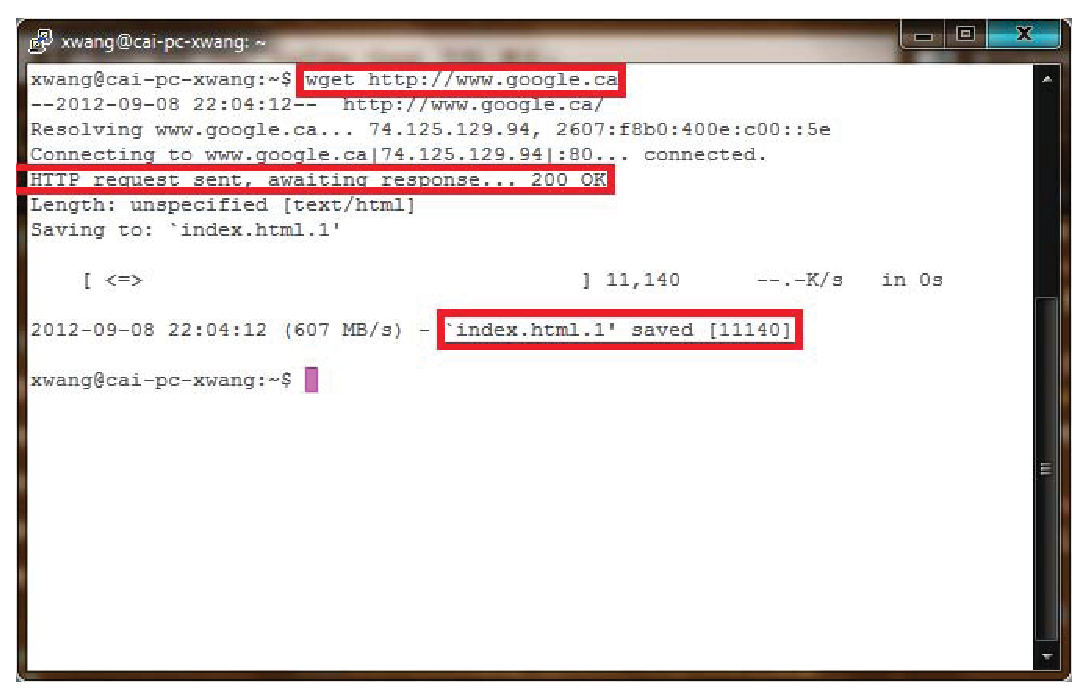
\includegraphics[width=0.8\columnwidth]{figs/lab_1_wget_url.eps}
\caption{Wget URL}\label{lab_1_wget_url}
\end{figure}

\item Close web browser. By minimizing browser activity you will stop your computer from fetching unnecessary web content, and avoid incidental traffic in the trace.

\item Launch Wireshark. Choose the network interface that we would
  like to capture the packets on. To do this, select ``Capture
  $\Rightarrow$ Options'' from the command menu. A window similar to
  the one shown in Fig.~\ref{lab_1_fig_2} should pop up. Select the
  interface you are using. Uncheck ``Capture packets in promiscuous 
  mode''. This mode is useful to overhear packets sent to/from other 
  computers on broadcast networks. We only want to record packets 
  sent to/from your computer. Use capture filter ``tcp port 80''. 
  This filter will record only standard web traffic and not other 
  kinds of packets that your computer may send. Click ``Start'' to 
  start the packet capture process.
 
\begin{figure}[!t]
\centering
\includegraphics[width=0.8\columnwidth]{figs/lab_1_fig_2.eps}
\caption{Capture options window}\label{lab_1_fig_2}
\end{figure}

\item When the capture is started, repeat the web fetch using wget above. This time, the packets will be recorded by Wireshark as the content is transferred.

\item After the fetch is successful, return to Wireshark and use the menus or buttons to stop the trace (``Capture $\Rightarrow$ Stop''). If you have succeeded, the upper Wireshark window will show multiple packets. How many packets being captured will depend on the size of the web page, but there should be at least 8 packets in the trace. An example is shown in Fig.~\ref{lab_1_wget_wireshark}.

\begin{figure}[!t]
\centering
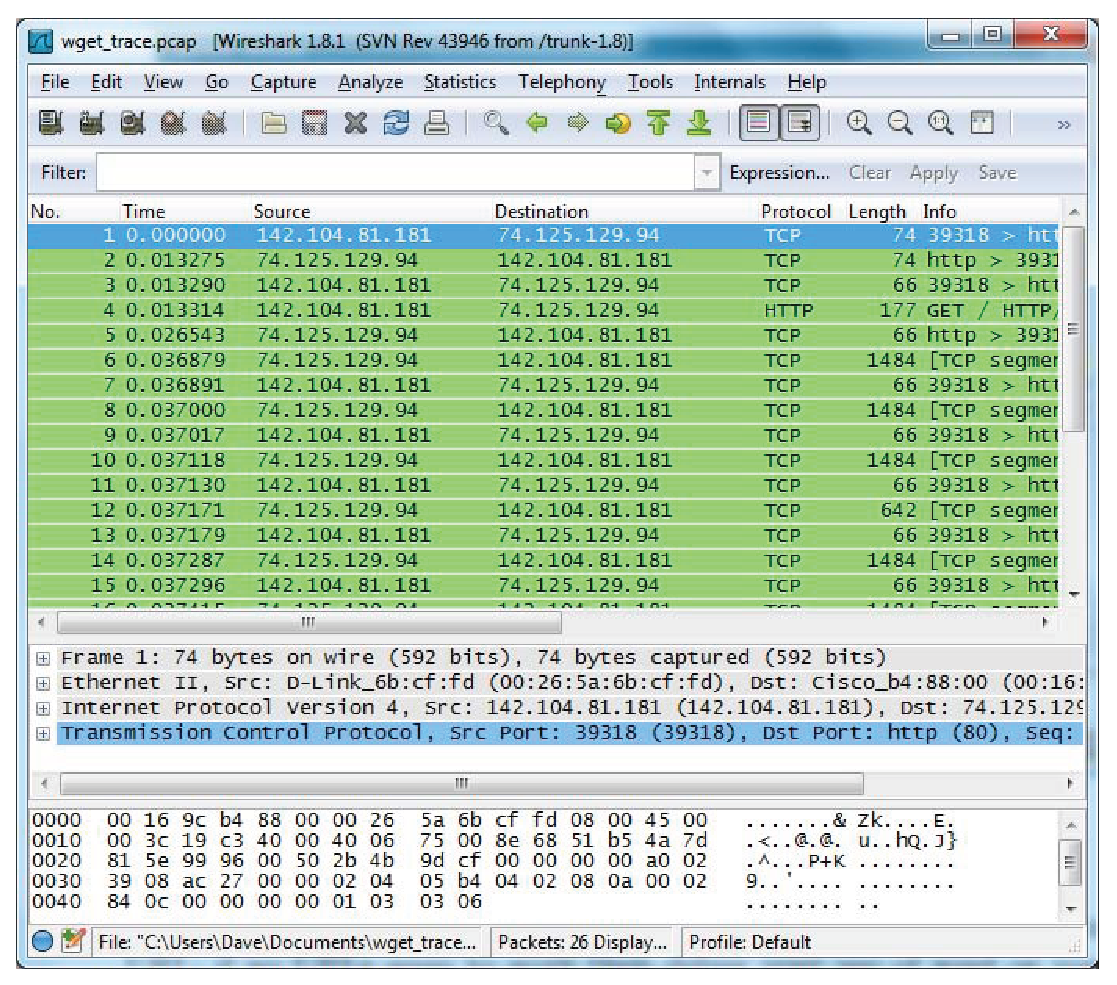
\includegraphics[width=0.8\columnwidth]{figs/lab_1_wget_wireshark.eps}
\caption{Packet trace}\label{lab_1_wget_wireshark}
\end{figure}

\end{itemize}

%\subsubsection{C.  Using traces}


\subsection{Layered Protocol}

%WireShark enables us to create and use traces. Traces are a set of
%captured packets that are saved in a file. In the following few
%experiments, we will use the existing traces to study how the HTTP
%protocol works.

By inspecting the captured trace, or the provided trace ({\bf lab1-wget-trace.pacp}) to understand the layered protocol.


\begin{itemize}
\item Select an HTTP GET packet. This packet carries the HTTP request sent
   from your computer to the server. 
   
\item The protocol layers being used in web fetching are shown in 
 Fig.~\ref{lab_1_protocol_stack_web}. HTTP is the application
 layer web protocol used to fetch URLs. It runs on top of the TCP/IP
  transport and network layer protocols. The link layer protocol shown in the 
  figure is Ethernet. It may be other protocol, depends on your network.   
  
\begin{figure}[!t]
\centering
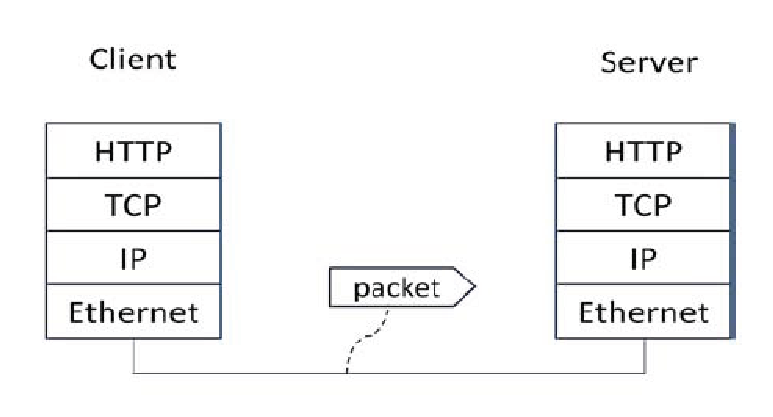
\includegraphics[width=0.8\columnwidth]{figs/lab_1_protocol_stack_web.eps}
\caption{Protocol stack for a web fetch}\label{lab_1_protocol_stack_web}
\end{figure}

\item Click on one HTTP packet, and turn to the middle panel with details of the packet. The first block is ``Frame''. This is a record that describes overall information about the packet, including when it was captured and how many bits long it is. The second block is ``Ethernet'' (You may have taken trace in a computer with 802.11, but still you will see an Ethernet block. This is because Wireshark capture traffic in Ethernet format determined on the capture options. See Link-layer header type.). Then we can see IP, TCP, and HTTP. This is a bottom-up order, because as packets are passed down the protocol stack, the header of the lower layer protocol is added to the front of the information from the higher layer protocol. That is, the lower layer protocols come first in the packet.

\item When an Ethernet frame arrives at a computer, the Ethernet layer must hand the packet that it contains to the next higher layer to be processed. In order to do this, the protocol use information in its header to determine the higher layer data unit encapsulated. Which field is used here?

\item Draw a figure of an HTTP GET packet that shows the position and size in bytes of the TCP, IP and Ethernet protocol headers. On this drawing, show the range of header and payload of each layer. 

\end{itemize}
 
\section{Discussion}

\subsection{Running WireShark}
\label{Dis_run_wireshark}

\begin{enumerate}

\item Capture a trace without filter.

\item List at least 3 different protocols that appear in the protocol
  column in the {\em unfiltered} packet-listing window.

\item How long did it take from the HTTP GET message being sent
  to the HTTP OK reply being received?

\end{enumerate}

\subsection{Networking Tools}

Explore the usage of ``ifconfig'', ``ping'', ``netstat'', and answer the following questions. (\textbf{Hint:} If you're not sure about how to use these commands, please check \textsl{Sec.~1.1.2 Networking Tools"}.)

\begin{enumerate}

\item  How many Ethernet interfaces are in your computer, how to determine it?

\item How to turn down/up an Ethernet interface?

\item Ping 10 packets to two websites. Compare the statistic results (packet loss, avg rtt).

\end{enumerate}

\subsection{Layered Protocol}

\begin{enumerate}

\item Draw the structure of a HTTP GET packet.

\item In the provided trace ({\bf lab1-wget-trace.pacp}), calculate the average overhead of \textbf{all} the packets \textbf{from the server to the client} (in percentage). ({\bf Hint:} For one packet, the overhead is the size of all headers in one packet over the total size. The average overhead is the ratio between total size of headers and total size of the packets).

\item Which Ethernet header field tells the next higher layer protocol is IP? What value it used?

\item Which IP header field tells the next higher layer protocol is TCP? What value it used?
\end{enumerate}

%\begin{thebibliography}{99}
%\bibitem{umass}Ethereal Labs,
%  http://www-net.cs.umass.edu/ethereal-labs
%\bibitem{wiki}Wikipedia.org,
%  http://en.wikipedia.org/wiki/HTTP
%\end{thebibliography}


\chapter{Lab 2: Ethernet and IEEE 802.11}\label{Lab2}

\section{Objective}
%List objectives of the lab
\noindent  In this lab, we will investigate the link layer protocols, including the Ethernet and IEEE 802.11. The first part of this lab is mainly about the Ethernet frame format. The second part of the lab focuses on analyzing IEEE 802.11 frames.

\section{Introduction}
%Introduce the theory behind what we are going to be doing in the lab
\subsection{Ethernet}
\noindent  Ethernet stations communicate by sending each other data frames. As with other IEEE 802 LANs, each Ethernet station is given a single 48-bit MAC address, which is used to specify the destination and the source of each data frame. Network interface cards~(NICs) or chips normally do not accept frames addressed to other Ethernet stations. Adapters are generally programmed with a globally unique MAC address, but this can be overridden, either to avoid an address change when an adapter is replaced, or to use locally administered addresses.\\

\noindent All generations of Ethernet~(except very early experimental versions) share the same frame formats~(and hence the same interface for higher layers), and can be readily~(and in most cases, cheaply) interconnected.\\

\noindent Due to the ubiquity of Ethernet, the ever-decreasing hardware cost of it, and the reduced panel space needed by twisted pair Ethernet, most manufacturers now build the functionality of an Ethernet card directly into PC motherboards, eliminating the need for installation of a separate network card.

\subsection{IEEE 802.11}
In this part, we are going to explore the link layer, and management functions of 802.11. Generally speaking, there are three types 802.11 frames, the Data frame~(Type 2), the Control frame~(Type 1), and the Management frame~(Type 0). For each type of frame, there are also different subtypes. Typically, Data frame is the longest, which can be up to 1500 bytes, while Management frames are much shorter, and Control frames are very short. As the Data and Control frames have been illustrated in the text book, here we introduce some important types of Management frames.

\begin{itemize}
\item \textbf{Beacon frame} Beacon frames are sent out periodically by an AP to advertise its existence and capabilities to nearby computers. Beacon is an IEEE 802.11 wireless LAN Management frame. In a Beacon frame, there are a series parameters, including the SSID name of the AP, the data rates it supports, and the channel on which it is operating. 

\item \textbf{Association} A computer has to associate with the AP after it learned an AP via a Beacon or otherwise and before it can send or receive data from the AP. Possibly, authentication process will be involved during the association. If the Association Request is successful received by AP, the AP will return an Association Response, and then the computer will acknowledge the association response. The Association Request and Response carry information that describes the capabilities of the AP and computer. Thus, both endpoints can know the other's abilities.

\item \textbf{Probe Request/Response} In addition to find AP by waiting to learn about an AP from Beacons, a computer may also probe for specific APs. A Probe Request is sent by a computer to test whether an AP with a specific SSID is nearby. If the AP is nearby, it will reply with a Probe Response. Like Beacon and Association frames, each of these frames carries information describing the capabilities of the computer and AP. 
\end{itemize}

\section{Procedures}
%List procedures of the lab
\subsection{Analyzing Ethernet frames}\label{Pro_Ethernet}
\begin{itemize}
\item Download and open the trace named ``ethernet-trace-1''.

%\item Because we are interested in Ethernet, we need not to consider any IP or higher layer protocols. Change WireShark's settings so that it shows information only about protocols below IP: select \textbf{\textsl{Analyze}} $\Rightarrow$ Enabled Protocols and unchecked ``IP''. The resulting figure should look like Figure~\ref{Lab2_fig_1}.

\item Find the HTTP GET message that was sent from the web browser to \url{gaia.cs.umass.edu}~(should be packet No.10) and answer question~(1)-(4) in section~\ref{Dis_Ethernet}.

\item Find the Ethernet frame containing the first byte of the HTTP response message and answer question~(5)-(8) in section~\ref{Dis_Ethernet}.
\end{itemize}

%\begin{figure}[ht]
%\centering
%\includegraphics[width=0.9\columnwidth]{Lab2_fig_1}
%\caption{Screen shot of WireShark}\label{Lab2_fig_1}
%\end{figure}

\subsection{Exploring IEEE 802.11 functions}\label{Pro_WLAN}
\begin{itemize}

\item Download and open the trace named ``wlan-trace-1''~\cite{Tanenbaum10}. Note that it may be difficult to gather your own trace using windows system. The main issue is that Windows system made 802.11 frames appear to come via a wired Ethernet. However, it is possible to use Mac or Linux to gather 802.11 frames directly, without this conversion.

\item Select a Data packet. The packet detail can show four layers information: 1)~Frame, which is a record added by Wireshark with information about the time and length of the frame; 2)~Radiotap, which is also a record of captured physical layer parameters, such as the strength of the signal and the modulation; 3)~IEEE 802.11, which is the bits of the 802.11 Data frame;4)~Data, which is a record containing the frame payload data. Answer the related questions in section~\ref{Dis_WLAN}. 

\item Inspect different packets to see the values for different types of frames. You can use filter to see only one type frames by entering the expression “wlan.fc.type$==$n” into the Filter box above the list of frames in the top panel. For example, "n=2" is for data frames, "n=1" is for control frames, and "n=0" is for management frames. Answer the related questions in section~\ref{Dis_WLAN}. 

\item Inspect the packet transmission reliability. Use filter expressions to find the number of Data frames that are originals and retransmissions. For example, “wlan.fc.type$==$2 $\&\&$ wlan.fc.retry$==$0” will find original Data frames. Answer the related questions in section~\ref{Dis_WLAN}. 

\item Inspect the Management frame. Use filter to help you find these frame, and answer the related questions in section~\ref{Dis_WLAN}. 
\end{itemize}

\section{Discussion}

\subsection{Analyzing Ethernet frames}\label{Dis_Ethernet}
\noindent For trace file ``ethernet-trace-1'', answer the following questions.
\begin{enumerate}
\item What is the 48-bit Ethernet address of the client computer?

\item What is the 48-bit destination address in the Ethernet frame? Is this the Ethernet address of \url{gaia.cs.umass.edu}? Which device has this as its Ethernet address?

\item Give the hexadecimal value for the two-byte Frame type field.

\item What is the value of the Ethernet source address? Is this the address of your computer, or of \url{gaia.cs.umass.edu} Which device has this as its Ethernet address?

\item What is the destination address in the Ethernet frame? Is this supposed to be the Ethernet address of the computer you are using?

\item Find the hexadecimal value for the two-byte Frame type field.

\end{enumerate}

\subsection{Exploring IEEE 802.11 functions}\label{Dis_WLAN}

\noindent Answer the following questions based on the trace file
``wlan-trace-1''.

\begin{enumerate}

\item Which AP is the most active one (i.e., the one sends most Beacon messages)? what is its BSS ID? 

\item How many Data frames are in the trace, how many subtypes, and what is the most common subtype of Data frame?

\item How many subtypes of Control frames are in the trace, what are they? and what is the most common subtype?

\item How many subtype of Management frames are in the trace, what are they and what is the most common subtype?

\item Please estimate the retransmission rate as the number of retransmissions (i.e., the total number of transmission - number of original frames) over the number of original transmissions. Show your calculation.

\item What are the Type and Subtype values for the Association Request/Association Response frames, the Probe Request/Probe Response frames?

\end{enumerate}

%\begin{thebibliography}{99}
%\bibitem{umass} Ethereal Labs,
%  http://www-net.cs.umass.edu/ethereal-labs
%\bibitem{wiki}Wikipedia.org, http://en.wikipedia.org/wiki/HTTP
%\end{thebibliography}



\chapter{Lab 3: ARP, IP, and ICMP}\label{Lab3}

\section{Objective}
%List objectives of the lab

\noindent In this lab, we will investigate the Address Resolution Protocol~(ARP), the IP~(Internet Protocol), and Internet Control Message Protocol~(ICMP). The first part of this lab is mainly about the ARP protocol. We will study the operation of the protocol based on the fields that it sets in the Ethernet frame containing the ARP message.  The second part of the lab focuses on analyzing IP frames, by observing and interpreting the fields in the IP frame. The last part of this lab focuses on the format and content of the ICMP messages.

\section{Introduction}
%Introduce the theory behind what we are going to be doing in the lab
\subsection{Address Resolution Protocol~(ARP)}
\par ARP is the standard method for finding a host's hardware address when only its network layer address is known.  It can be used to resolve many different network-layer protocol addresses to hardware addresses. Due to the overwhelming prevalence of IPv4 and Ethernet, ARP is primarily used to translate IP addresses to Ethernet MAC addresses. ARP is used in the following four cases when two hosts communicate:
\begin{enumerate}

\item When two hosts are on the same network and one desires to send a packet to the other.

\item When two hosts are on different networks and must use a gateway/router to reach the other host.

\item When a router needs to forward a packet for one host through another router.

\item When a router needs to forward a packet from one host to the destination host on the same network.
\end{enumerate}

\noindent The first case is used when two hosts are on the same physical network (that is, they can directly communicate without going through a router). The last three cases are the most used over the Internet as two computers on the Internet are typically separated by several hops.

\subsection{Internet Protocol~(IP)}
\par Above the link layer, there is the network layer, which is responsible for relay the date between the transport layer and the link layer. The network protocol in network layer is called the Internet Protocol, or more commonly, the IP Protocol. The IP protocol performs two basic functions, the addressing~(IP address) and the packet routing. Note that the internet layer is agnostic of application data structures as the transport layer, and it also does not distinguish between operation of the various transport layer protocols. Thus, IP protocol can carry data for a variety of different upper layer protocols by different protocol numbers, such as TCP, UDP and ICMP. \\

\noindent There are currently two versions of the IP protocol, IPv4 and IPv6. In this section we examine IPv4, which the most widespread version. With given trace files, we're going to learn about the details of IP frame. 

\subsection{Internet Control Message Protocol~(ICMP)}
\par The Internet Control Message Protocol~(ICMP) is one of the core protocols for network management in the Internet. It is mainly used by networked computers' operating systems to send error messages — indicating, for instance, that a requested service is not available or that a host or router could not be reached. It has been used in network trouble-shooting and analyzing applications such as \textit{ping} and \textit{traceroute}.\\

\noindent ICMP uses the basic support of IP as if it were a higher level protocol; however, ICMP is actually an integral part of IP, and must be implemented by every IP module. ICMP messages are sent in several situations: for example, when a datagram cannot reach its destination, when the gateway does not have the buffering capacity to forward a datagram, and when the gateway can direct the host to send traffic on a shorter route~[RFC792].\\

\noindent In this part of the lab, we use two network tools. One is \textit{ping}, which is used to test whether a particular host is reachable across an IP network, to self-test the network interface card of the computer, or to measure latency. The other one is \textit{traceroute}, used to determine the route taken by packets across an IP network.  We can understand the functions of ICMP by using these tools.

\section{Procedures}
%List procedures of the lab
\subsection{Exploring ARP functions}\label{Pro_ARQ}
\begin{itemize}
\item Download and open the trace named ``ethernet-trace-1''.

\item This trace basically emulates retrieving a long document.

\item The ARP protocol typically maintains a cache of IP-to-Ethernet address translation pairs on your computer.

\item Find the ARP request message and answer questions~(1)-(5) in section~\ref{Dis_ARP}.

\item Find the ARP reply that was sent in response to the ARP request and answer questions~(6)-(10) in section~\ref{Dis_ARP}.
\end{itemize}

\subsection{Analyzing IP frames}\label{Pro_IP}
\begin{itemize}
\item Using the same trace file as above.

\item Select any packet with the HTTP GET message in the trace and expand the IP header fields~(using the “+” expander or icon) to see the details. You can simply click on a packet to select it~(in the top panel). And the details of its structure~(in the middle panel) and the bytes that make up the packet~(in the bottom panel). Our interest is the IP header, and you may ignore the other higher and lower layer protocols. 

\item Select the the packet with HTTP GET message~(the No.10 packet) and answer questions~(1)-(2) in section~\ref{Dis_IP}.

\item Observe all the packets and answer questions~(3)-(4) in section~\ref{Dis_IP}.
\end{itemize}

\subsection{Exploring ICMP functions}\label{Pro_ICMP}
A. {\em Ping} The {\em ping} program in the source host sends a packet to the target IP address; if the target is alive, the {\em ping} program in the target host responds by sending a packet back to the source host. Both of these {\em ping} packets carry ICMP messages.\\

\noindent The following procedures describe how to capture the traces of ping messages.
\begin{itemize}
\item Start up the WireShark and begin packet capture.
 
\item Open a console, type the command \textit{ping www.engr.uvic.ca -c 10\footnote{The \textsl{ping} command here is different in Linux and Windows operating system. If you're working in Windows system, the command here should be \textsl{ping www.engr.uvic.ca -n 10}}} in the command line. The argument ``-c 10'' indicates that ten ping messages should be sent.

\item When the {\em ping} program terminates, stop the packet capture.

\end{itemize}

\noindent Download and open ``ping-trace-1'' in WireShark. Use the display filter to list the ICMP messages only, as shown in Figure~\ref{Lab3_fig_1} and answer questions~(1)-(4) in section~\ref{Dis_ICMP}.
\begin{figure}[hbt]
\centering
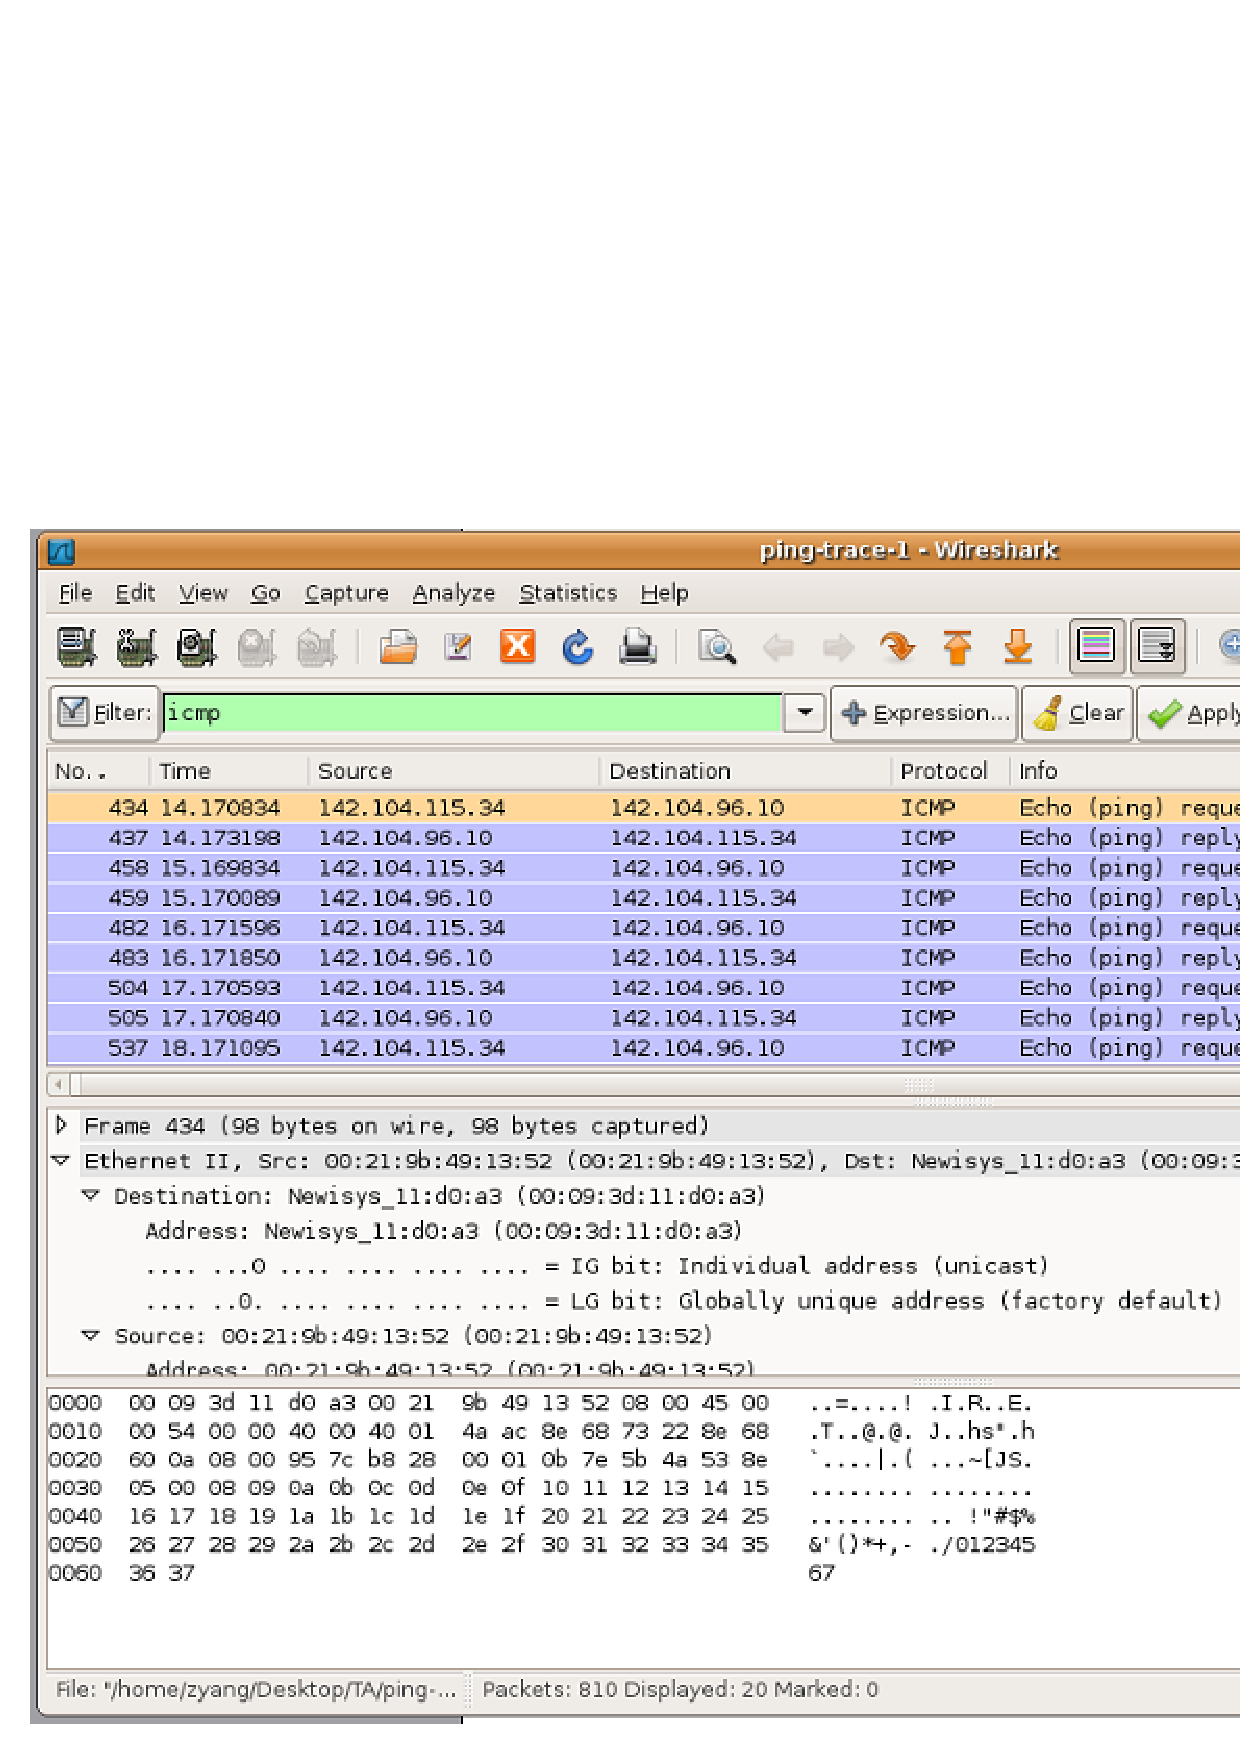
\includegraphics[width=5.5 in,angle=0]{Lab3_fig_1}
\caption{Capture of {\em ping} packet with ICMP display filter} \label{Lab3_fig_1}
\end{figure} \\

\noindent B. {\em Traceroute} The {\em traceroute} program is used to figure out the path a packet takes from the source to the destination. The following procedures describe how to capture the packets of traceroute messages.

\begin{itemize}
\item Start up the WireShark and begin packet capture.

\item Open a console, type the command \textit{traceroute www.engr.uvic.ca} in command line.

\item When the \textit{traceroute} program terminates, stop the packet capture.

\end{itemize}

\noindent Download and open ``tracert-trace-2'' in WireShark, and set the display filter as \textit{icmp}. Then answer the questions~(5)-(7) in section~\ref{Dis_ICMP} based on the trace.

\section{Discussion}

\subsection{Exploring ARP functions}\label{Dis_ARP}
\noindent  Answer the following questions based on the trace file ``ethernet-trace-1''.

\begin{enumerate}

\item What are the hexadecimal values for the source and destination addresses in the Ethernet frame containing the ARP request message?

\item Find the hexadecimal value for the two-byte Ethernet Frame type field. 

%\item What do the bit(s) whose value is $1$ mean within the flag field?

%   \item Discribe the content of the Ethernet frame (containing the ARP message). What are the values and meanings of these fileds?

\item  Where the ARP opcode~(operation code) field is located, i.e., how many bytes bits are there between of first bit of the opcode and the first bit of the ARP message?
%How many bytes from the very beginning of the Ethernet frame does the ARP opcode field begin?

\item What is the value of the opcode field within the ARP-payload part of the Ethernet frame, in which an ARP request is made?

\item Does the ARP message contain the IP address of the sender?
   
%\item Which field contains the MAC address of the host whose corresponding IP address is being queried, and what is it?

\item Where the ARP opcode field is located, i.e., how many bytes from the very beginning of the Ethernet frame does the ARP opcode field begin?

\item What is the value of the opcode field within the ARP-payload part of the Ethernet frame in which an ARP response is made?
      
\item What is the MAC address answered to the earlier ARP query?
      
\item What are the hexadecimal values for the source and destination addresses in the Ethernet frame containing the ARP reply message?
  
\item Why there is no ARP reply for the second ARP query~(packet No.6)?
\end{enumerate}

\subsection{Analyzing IP frames}\label{Dis_IP}
Answer following questions based on ``ethernet-trace-1''.
\begin{enumerate}

\item Sketch a figure of \textbf{the packet you selected} to show the position and size in bytes of the IP header fields, as well as the values in hexadecimal. Your figure can simply show the frame as a long, thin rectangle. 
	
\item What are the IP and MAC addresses of the source and destination?
	
\item How does the value of the Identification field change or stay the same for different packets? Is there any pattern if the value does change?	
	
\item How can you tell from looking at a packet that it has not been fragmented? 
\end{enumerate}

\subsection{Exploring ICMP functions}\label{Dis_ICMP}
Answer following question based on ``ping-trace-1'' and ``tracert-trace-2''.

\begin{enumerate}
\item What is the IP address of the source host~(client)? What is the IP address of the destination host~(server)?

\item  Can you get the average RTT (Round Trip Time)? What's that?

\item Examine one of the ping request packets. What are the ICMP type and code numbers? What other fields does this ICMP packet have? How many bytes are the checksum, sequence number and identifier fields?

\item Examine the corresponding ping reply packet. What are the ICMP type and code numbers? What other fields does this ICMP packet have? How many bytes are the checksum, sequence number and identifier fields?\\

\item What is the IP address of the source host~(client)? What is the IP address of the destination host~(server).

%\item Is there any difference between the request and reply packets from ``ping-trace-1'' and ``tracert-trace-2''? Why so?

\item Examine the ICMP error packet, which could be found in the
  packets from \textit{tracert-trace-2}. It has more fields than the
  ICMP echo packet. What are included in those fields? Find the TTL
  field, and explain what is it?

\item How many routers are between the source and the destination~(\textsl{www.engr.uvic.ca}), for the trace file? Please draw a figure to show the sequences of these routers, i.e, source --$>$ router\_\textsl{first} --$>$ ... --$>$ router\_\textsl{last} --$>$ destination?

\item Can you get the average RTT times between the source host and each router? What are they?

\end{enumerate}



\chapter{Lab 4: TCP}

\section{Objective}

\hspace*{0.5cm} In this lab, we first get familiar with the format of
TCP header, then study the TCP 3-Way Handshake and reliable
data transfer, followed by the congestion
control algorithm and retransmission scheme.

\section{Introduction}

\hspace*{0.5cm} TCP is the dominant
transport layer protocol in the Internet. It provides a reliable, in-order
stream of data between two end-points, even if they
are connected by a network that may drop, re-order, or corrupt the
packets. TCP provides the reliable data streaming service by detecting if
packets are lost, delayed, or corrupted during transmission.

In this Lab and the following Lab, we investigate the behaviour of TCP
in detail, by analysing a trace of the TCP segments sent
and received in transferring a $300$~KB file from a local computer (the
client, IP address: 10.0.1.5) to a remote Web server
(\url{http://gaia.cs.umass.edu/}, IP address: 128.119.245.12). The
file, named alice.txt (which contains two copies of the text of {\em
  Alice in Wonderland}) is stored on the client computer and is
uploaded to the server using the HTTP POST method. Here the POST
method is used in order to transfer a large amount of data from a
computer to another computer.

The procedure to transfer this file is as follows:

\begin{itemize}
\item Start up Web browser on the client computer and go to
  \url{http://gaia.cs.umass.edu/ethereal-labs/TCP-ethereal-file1.html}.
  The screen looks like Figure~\ref{lab_4_fig_1}.
\begin{figure}[ht]
    \centering
    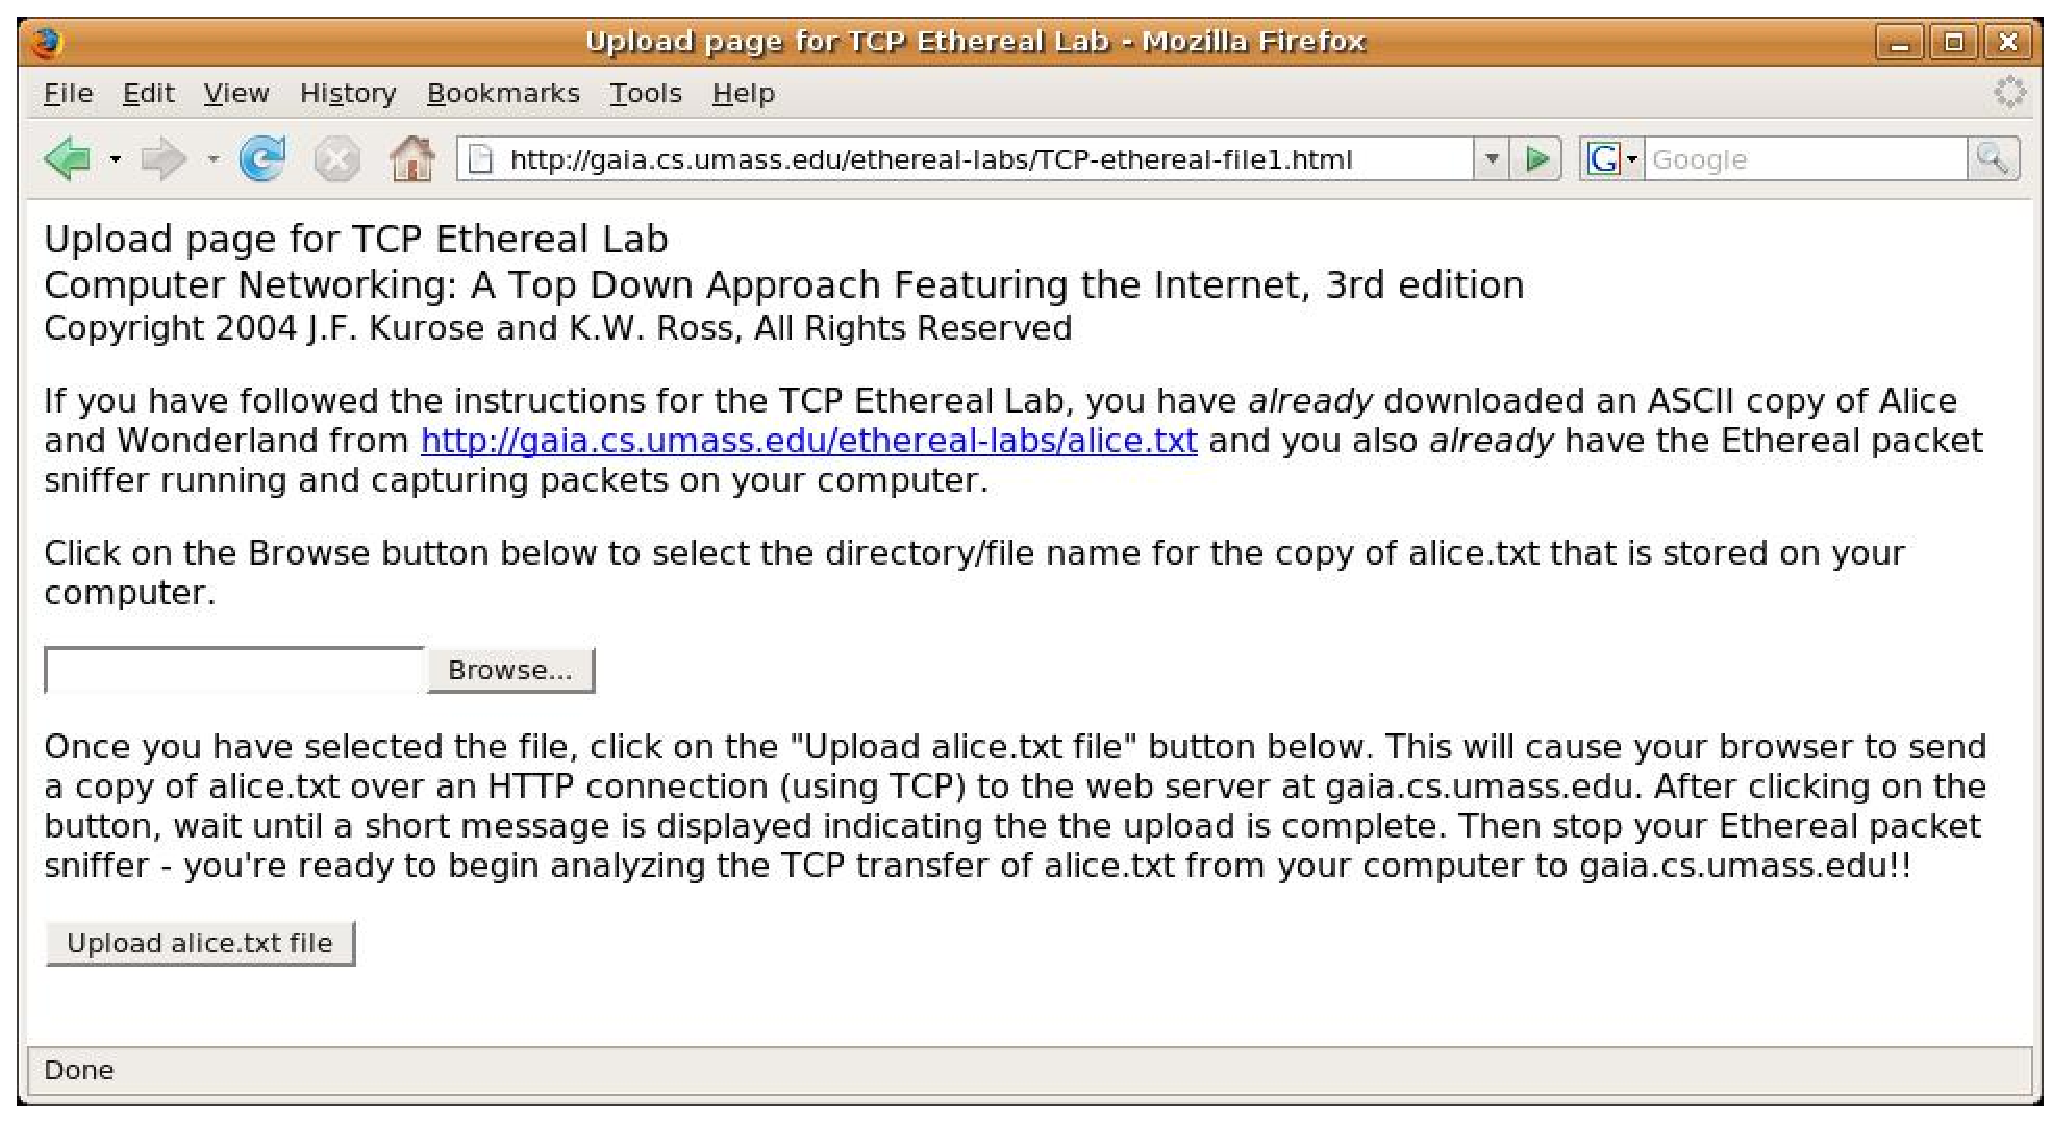
\includegraphics[width=0.99\columnwidth]{figs/lab_4_fig_1.eps}
    %\includegraphics[width=0.99\columnwidth]{lab_2_fig_1.jpg}
    \caption{Upload page}\label{lab_4_fig_1}
\end{figure}
\item Use the {\em Browse} button to enter the full
  path name of alice.txt on the client computer, and then press the
  {\em Upload alice.txt file} button to upload the file to the server
 \url{gaia.cs.umass.edu}.
\item Once the file has been uploaded, a new web page, which is a
  short congratulation, will be transferred from the Web server to the
  client and displayed in the web browser, as shown in Figure~\ref{lab_4_fig_2}.
\begin{figure}[ht]
    \centering
    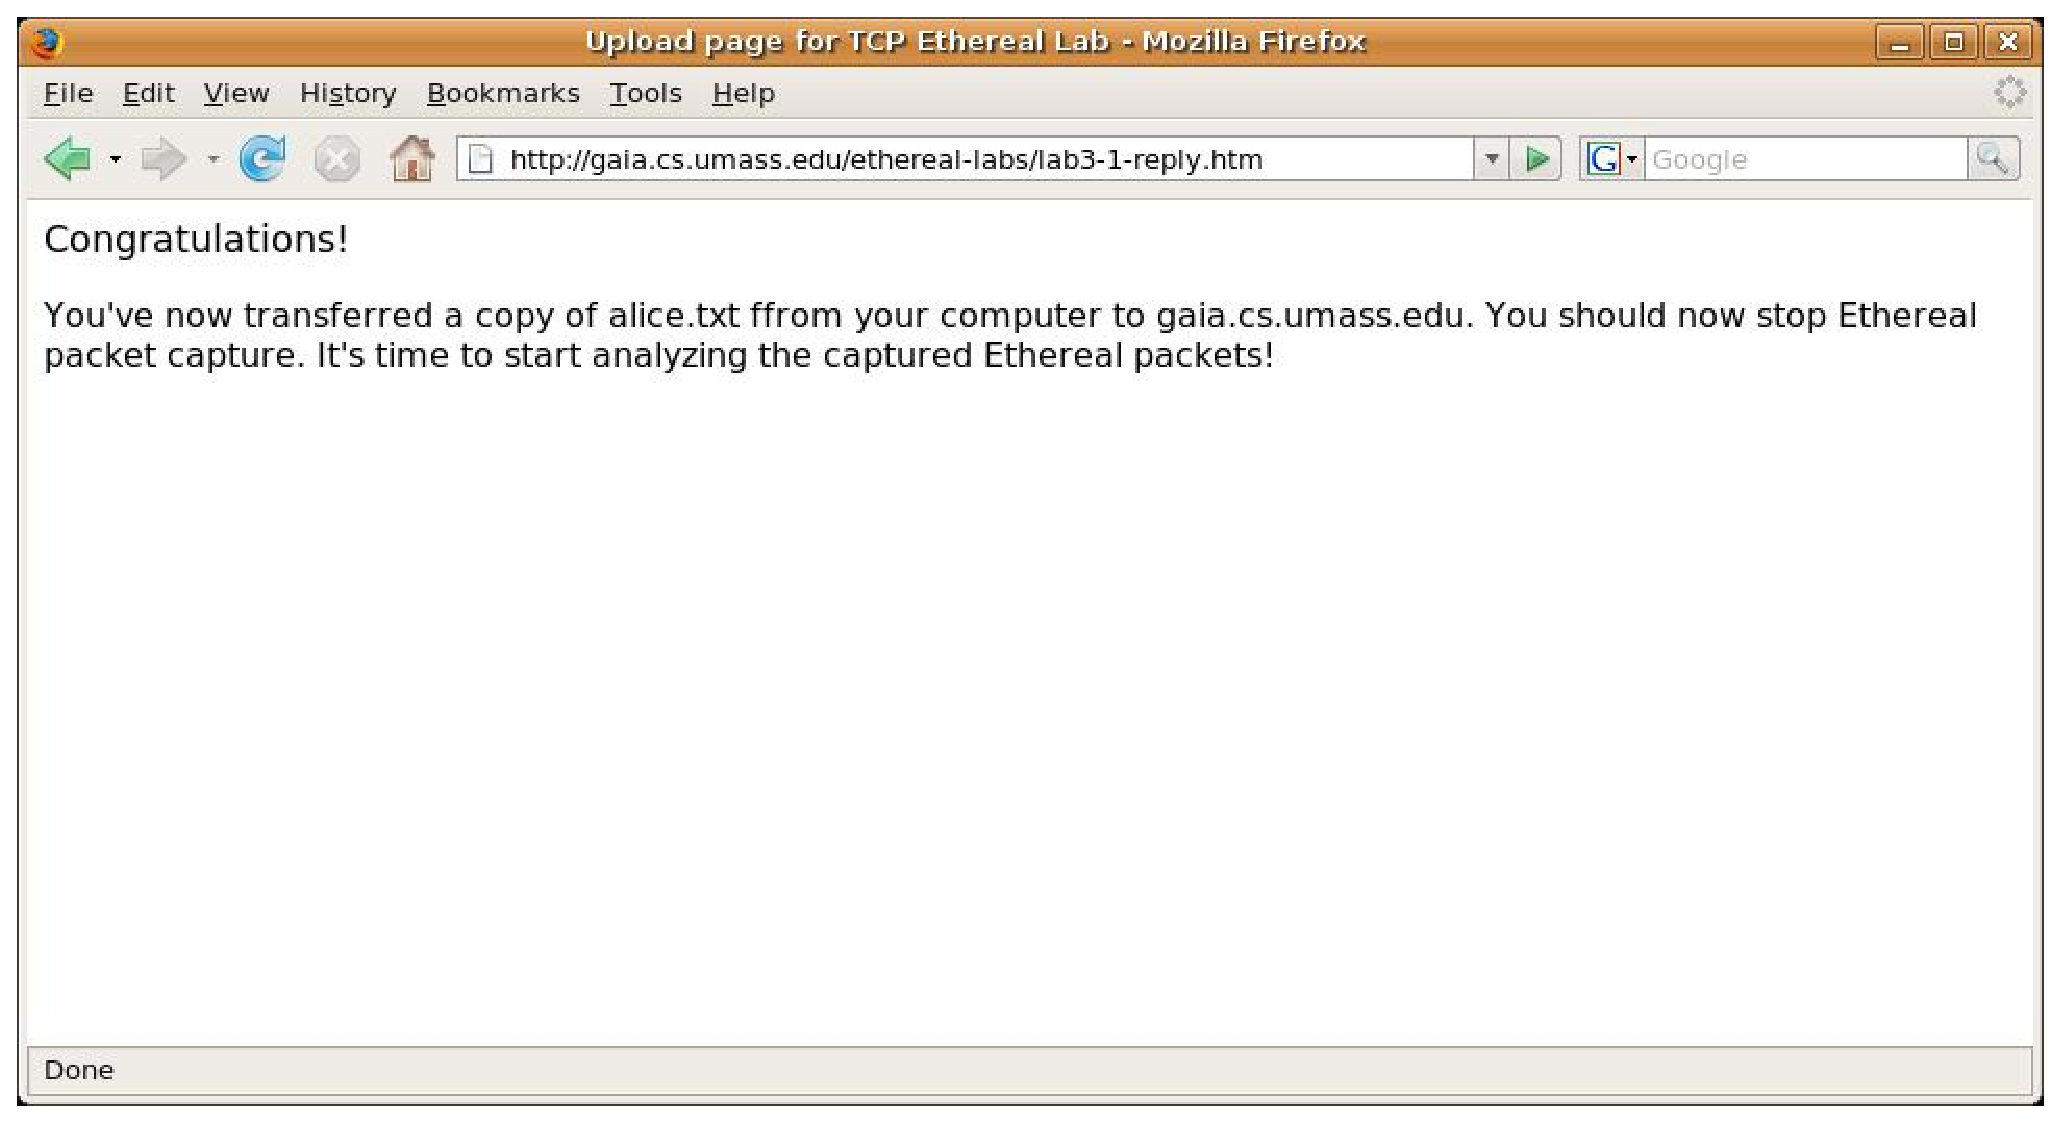
\includegraphics[width=0.99\columnwidth]{figs/lab_4_fig_2.eps}
    %\includegraphics[width=0.99\columnwidth]{lab_2_fig_2.jpg}
    \caption{Congratulation Page}\label{lab_4_fig_2}
\end{figure}
\end{itemize}

To transfer alice.txt and the congratulation page without
error, a TCP connection between the client and the server is
established.  The TCP connection completes the four operations in this
real-world application as follows:

\begin{itemize}
    \item TCP connection setup.
    \item Transfer the HTTP POST command and the file alice.txt, from
      the client computer to the server \url{gaia.cs.umass.edu}.
    \item Transfer the congratulation page from the server to the client.
    \item TCP connection release.
\end{itemize}

WireShark is run on the client computer to capture the trace of the
TCP segments sent/received from/to the client computer while the
file is being transferred. We saved the trace from the TCP stream in
the file {\bf tcp-trace-1.cap}. The trace tracked all of the above
four actions of TCP. We use this trace to study the 
TCP behaviours in this lab.

\subsection{TCP Header Format}

\hspace*{0.5cm} Every TCP segment consists of a header followed by an
optional data portion. The format of the header is defined in RFC 793,
including Source Port (16 bits), Destination Port (16 bits), Sequence
Number (32 bits), ACK (32 bits), .... In this lab, we will see the
details of the TCP headers used in this 
application.

\subsection{TCP Connection Setup}

\hspace*{0.5cm} Before transferring data, a TCP connection is
established between the two end systems, typically with  three messages,
called the three-way handshake: SYN $\rightarrow$ SYNACK $\rightarrow$
ACK.  The handshake is also used to negotiate certain properties of
the connection, e.g., the Maximum Segment Size (MSS) that the client
and server can accept, and the Selective Acknowledgement (SACK)
option.  In this lab, we will see the three-way handshake procedure in
the trace {\bf tcp-trace-1.cap}.%  The initial sequence number for
% each direction and some properties were set in the three-way
% handshake.

\subsection{TCP Data Flow}

\hspace*{0.5cm} Once the connection is established, the TCP sender
partitions the message from the application into segments. The MSS is
used to determine how to partition the single message so the
underlying network can encapsulate each segment into a packet without
further fragmentation.  The sequence number and ACK number are used to
detect packet loss, duplication, re-order in transmission and to
deliver the segments correctly and in-order to the application in the
destination host.

In this real-world application, after the connection was established,
the client computer wrote about 300KB into the data stream using
the HTTP POST command. From the application's perspective, this was
sent as one unit, or one message. However, the underlying network
cannot support packets large enough to hold all 300KB of
data. We will see that TCP broke this single logical transmission into
multiple segments according to MSS.

In the trace file {\bf tcp-trace-1.cap}, the first three segments are
used to establish the connection. Starting from the No.4 TCP segment,
the client  began to transfer the application layer message to
the server. The 4th segment contains the HTTP POST command (we will
dig into the packet content field and see this HTTP command).  This
segment is actually used to transfer this HTTP command. The text file
is transferred by the following TCP segments. Here we regard both the
HTTP POST command and the file (alice.txt) together as the whole
message. Therefore, we consider the 4th TCP segment as the first
segment in the TCP connection to transfer the message from the
client to the server.

\subsection{TCP Connection Release}

\hspace*{0.5cm} The TCP connection is closed when the two end systems
exchange TCP segments with FIN bit set and ACKed by the other side.
The FIN bit literally means that no additional new data will be sent
on that side of the connection.

The sequence of two FINs and their corresponding ACKs is the preferred
way to gracefully terminate a TCP connection. However, TCP connections
can also be terminated by setting the RESET bit.  Although the RESET
was designed to be used for unrecoverable errors, it is often used in
practice for fast termination that avoids the formalities of the
FIN-ACK exchanges.

In the trace file {\bf tcp-trace-1.cap}, after the client
acknowledged the data of the congratulation page, the server sent a
FIN indicating that it would not be sending any additional data. The
client acknowledged this FIN by sending back the ACK. Therefore the
flow in the direction from the serve to the client is closed. The
client computer could also terminate its flow to the server by
sending the FIN segments. Alternatively, the client computer 
sent a RESET segment to the server to release the connection.



\subsection{TCP Congestion Control (Optional)} 

\hspace*{0.5cm} In TCP, congestion control provides the ability to
limit the sending rate in response to signs of network congestion.
Congestion control helps the network to recover from congestion by
shrinking sender's outgoing traffic and therefore avoids network
congestion collapse, and at the same time tries to achieve
throughput as high as possible.

Congestion control is realized by setting the size of congestion
window, according to two strategies, the slow start and the congestion
avoidance. During the slow start phase, the congestion window increases 
one MSS with each acknowledgement, and subsequently 
the window size is doubled every round-trip time (RTT). During congestion
avoidance, each acknowledgement increases the congestion window by
$MSS^2/ congestion\ window\ size$ (if the receiver sends ACK for each
received packet without delay), and subsequently the congestion window
size is increased by one MSS every RTT. Slow start phase changes to
congestion avoidance phase when congestion window exceeds the
slow-start threshold.

We will use the TCP segment trace file,
\textbf{tcp-trace-1.cap} to
investigate TCP congestion control. In particular, we 
look at how the congestion window evolved since the beginning of
transferring the HTTP POST command and the alice.txt file.

\subsection{TCP Flow Control (Optional)}

\hspace*{0.5cm} TCP also provides flow control or the ability to limit
the sending rate to avoid a fast
sender over-running a slow receiver. To provide a reliable service,
a TCP receiver cannot deliver data that it received out of order to
the waiting application. Therefore, the TCP receiver typically
allocates a fixed amount of buffer space to store both out-of-order
data and data waiting for the application to fetch. If the TCP
receiver runs out of buffer space to hold the incoming data, then it
has no choice but to drop the out-of-order data packet even
if it is error-free.

The receiver advertises its available buffer in each acknowledgement.
The receiver's advertised window field is used to inform the sender
how much room is left for the incoming data. Then in the sliding-window
based flow control, the sender chooses the minimum of the receiver
window and the congestion window to be the size of the sliding window in
order to make sure that the receiver will not run out of buffer
space.

In this subsection, we will still use the TCP segment trace file,
\textbf{tcp-trace-1.cap}, to exam TCP flow control. We will see that
the receiver window took effect and throttled the sender even though
the congestion window continued to grow.

\subsection{Retransmission in TCP}

\hspace*{0.5cm} We learned that TCP provides reliable data
transmission over an unreliable network by relying on feedback from
the receiver to detect loss and responding to packet loss with
retransmissions. TCP uses two kinds of indications of packet losses,
time-out and duplicated acknowledgement (which is regarded as an early
indication of packet loss and causes the fast retransmission instead
of waiting until timeout). The TCP sender must maintain a copy of the
data it sent in case retransmission is needed, so it must store the
data until the corresponding acknowledgement is received.

However, in the trace \textbf{tcp-trace-1.cap}, all the packets were
received correctly the first time and thus there was no
retransmission. In order to investigate the TCP retransmission
scheme, we are going to analyse another trace of TCP connections,
\textbf{tcp-trace-retransmission.cap}~\cite{Matthews04}, in which
retransmission does occur.

The trace, \textbf{tcp-trace-retransmission.cap}, was taken on a
private network~\cite{Matthews04}. A desktop PC and a laptop were
connected via a wireless router. The laptop was connected via a
wireless interface and specifically placed so as to interfere with a
strong signal. The IP addresses of the desktop and the laptop are,
respectively, 192.168.0.100 and 192.168.0.102. The desktop sent a file
(about 40K bytes) to the laptop using TCP. The TCP port number for the
desktop is 4480, and 5001 for the laptop. The experiment configuration
is shown in Figure~\ref{lab_4_fig_config}. WireShark was run on the sender,
i.e., the desktop, while the file was being transferred to capture the
TCP segments exchanged. The TCP connection trace was saved in file
\textbf{tcp-trace-retransmission.cap}.

\begin{figure}[ht]
    \centering
    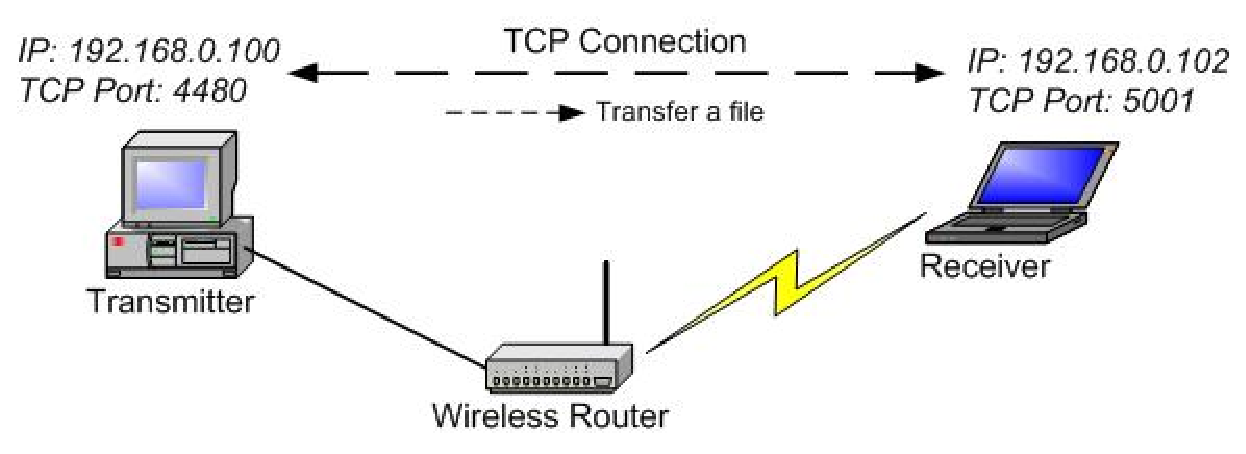
\includegraphics[width=0.99\columnwidth]{figs/lab_4_network_configuration.eps}
    %\includegraphics[width=0.99\columnwidth]{lab_2_fig_1.jpg}
    \caption{Network Configuration}\label{lab_4_fig_config}
\end{figure}

In this lab, we will take a look at both the fast retransmission and
the time out retransmission using this trace file.

\section{Procedures}

{\bf Note:}  You will answer a set of questions by exploring the 
trace file {\bf tcp-trace-1.cap} and {\bf tcp.analysis.retransmission.cap}.
 Whenever possible, when answering a 
question you should provide the information of the packet(s) within 
the trace that you used to answer the question asked. The information 
includes the Packet No., the name(s) and value(s) of the packet field(s) 
that you use to answer the questions.

\subsection{TCP Header Format}
\begin{itemize}
\item Download the traces folder from the lab website.

\item Open the captured trace file named {\bf tcp-trace-1.cap} with
  WireShark.  Now what you should see is a series of TCP segments sent
  between the client  and the server \url{gaia.cs.umass.edu}.

\item Since this lab is about TCP rather than HTTP, change WireShark's
  {\em Packet List Pane} window so that it shows information about the
  TCP segments containing the HTTP messages.
  % , rather than about the HTTP messages.
  To do this, in WireShark, select {\em Analyze $\Rightarrow$ Enabled
    Protocols}. Then uncheck the {\em HTTP box} and select {\em OK}.
\item Select the first packet and explore the details of the TCP
  segment using the {\em packet details pane} and the {\em packet bytes
  pane}.
\item Select the {\em Transmission Control Protocol} item in the
  \emph{Packet Details Pane} then the content of the header is
  highlighted in the {\em Packet Bytes Pane}.
  % port 80 => Hex 0050, 4335 => Hex 10ef
\item Answer the related questions in section \ref{sec:tcp-head}.

\end{itemize}

\subsection{TCP Connection Setup}

\begin{itemize}
\item Find the initial three-way handshake in the trace file. (Hint: 
  You should see the SYN segment sent from the client to 
  \url{gaia.cs.umass.edu}, and also the SYNACK segment being returned.)
\item Answer the related questions in section \ref{sec:tcp-con}.
\end{itemize}

\subsection{TCP Data Flow}

\begin{itemize}
\item Check the HTTP POST command. Select the 4th segment in the {\em
    Packet List Pane}. Select the {\em Data} item in the {\em Packet
    Details Pane} and the content of the data carried by this segment
  is highlighted in the {\em Packet Bytes Pane}. You should find a
  POST and other HTTP command information within its {\em Date} field.

\item Set time reference. In order to make the following analysis
  easier, set time reference to the 4th packet. Choose the {\em Time
    Reference} items in the {\em Edit} menu, or from the pop-up menu
  of the {\em Packet List Pane}.

  {\bf Note:} Now the 4th packet becomes the starting point for all
  subsequent packets. The time values of all the following packets are
  calculated relative to this packet.

\item Set the time display format as microseconds. Choose the {\em
    Time Display Format} in the {\em View} menu. Then select {\em
    Seconds Since Beginning of Capture} and {\em Microseconds}.

\item Answer the related questions in section \ref{sec:2.4.3}.
\end{itemize}

\subsection{TCP Connection Release}

\begin{itemize}
\item Find the segments used to release the connection between the 
client and the server.
\item Answer the related questions in section \ref{sec:2.4.4}.
\end{itemize}



\subsection{TCP Congestion Control}\label{sec:3.3.1}

\begin{itemize}
  \item Download the HTTP traces folder from the lab website.
  \item Open the captured trace file named \textbf{tcp-trace-1.cap}
    with WireShark.
  \item Since this lab is about TCP rather than HTTP, change
    WireShark's {\em Packet List Pane} window so that it shows
    information about the TCP segments containing the HTTP messages.
    To do this, select {\em Analyze $\Rightarrow$ Enabled Protocols}.
    Then uncheck the {\em HTTP box} and select {\em OK}.
  \item Set time reference. In order to make the following analysis
    easier, set time reference to the 4th packet. Choose the {\em Time
      Reference} items in the {\em Edit} menu, or from the pop-up menu
    of the {\em Packet List Pane}.
  \item Answer the related questions in section \ref{sec:3.4.1}.
\end{itemize}

\subsection{TCP Flow Control}\label{sec:3.3.2}

\begin{itemize}
\item Open the captured trace file named {\bf tcp-trace-1.cap} with
  WireShark.
\item Answer the related questions in section \ref{sec:3.4.2}.
\end{itemize}

\subsection{Retransmission in TCP (Optional)}\label{sec:3.3.3}

\begin{itemize}
\item Open the captured trace file named
  \textbf{tcp-trace-retransmission.cap} with WireShark.
\item List retransmissions. Search for retransmissions with the
  display filter \emph{tcp.analysis.retransmission}. Applying this
  filter, you should see 9 retransmissions in the trace.
\item Answer the related questions in section \ref{sec:3.4.3}.
\end{itemize}

\section{Discussion}

\subsection{TCP Header Format}\label{sec:tcp-head}

\begin{enumerate}
\item Write down the TCP header content in hexadecimal format (in the
  {\em packet bytes pane}). Dissect the TCP header and indicate the
  value of each field in the header. Annotate the
  hexadecimal content to explain your answer.
\item What are TCP port numbers used by the client computer (source)
  and the server (destination) when transferring the file to
  \url{gaia.cs.umass.edu}? How did the client computer determine the
  port numbers when it wanted to set up a TCP connection to the
  server?
\item What is the maximum header length? Given the value of the Header
  Length field, how to calculate the length of the head in unit of
  bytes? Verify your answer using the first TCP segment in the trace
  file.
\item (Optional) How does TCP calculate the Checksum field? What is
  the pseudo-header format? Write down the pseudo-header of the flow
  from the client to the server in hexadecimal format. Verify the
  Checksum value in the first TCP segment in the trace file.
% c: too time-consuming
\end{enumerate}

\subsection{TCP Connection Setup} \label{sec:tcp-con}
\begin{enumerate}
\item Which segments are the initial three-way handshake in the trace
  file? How do you determine this?
\item What is the actual initial sequence number in each direction (in
  hexadecimal format)? How did the client  and the server
  determine these values?

  {\bf Note:} WireShark displays the relative sequence number. You
  should select the {\em Sequence Number} field in the header, the
  actual value is highlighted in the {\em Packet Bytes Pane}.

\item What is the value of the acknowledgement number in the SYNACK
  segment? How did \url{gaia.cs.umass.edu} determine that value?

\item What are the values of the sequence number and the
  acknowledgement number in the third ACK segments in the three-way
  handshake? How did the client computer determine these values?

\item How did the client and the server announce the maximum
  TCP payload size that they were willing to accept? What are the
  values and why did they choose these values?

\item Is there data sent in the SYN, SYNACK, and ACK segment? How do
  you determine this?
\end{enumerate}

\subsection{TCP Data Flow}\label{sec:2.4.3}
\begin{enumerate}
\item Beginning with the 4th segment, what are the sequence number,
  acknowledgement number, data length, and the time of the segment
  sent/received from/to the client computer of the 4th, 5th, 6th, ...,
  15th segments in the TCP connection? Fill out Table~\ref{lab_2_tab_1} for the data
  flow from the client computer to the server. ({\bf Note:} list both the actual
  value and relative value of the sequence number and acknowledgement
  number.)
\begin{table}[ht]
    \centering
    \includegraphics[width=0.75\columnwidth]{figs/lab_4_table_1.eps}
    %\includegraphics[width=0.99\columnwidth]{lab_2_fig_1.jpg}
    \caption{TCP segment exchange table (Please show the segment and its acknowledgement in the same row.)}\label{lab_2_tab_1}
\end{table}

\item What are the segments acknowledged by the packet 6, 9, 12, and
  15, respectively? ({\bf Hint:} acknowledgement number is the next
  byte expected, so it actually acknowledges the bytes before the
  acknowledgement number.)

\item Given the difference between when each TCP segment was sent, and
  when its acknowledgement was received, what is the RTT value for each
  of the segments which have been acknowledged before the 15th
  segment?

\item (Optional) What is the Estimated RTT value after the receipt of
  each ACK?  Assume that the value of the Estimated RTT is equal to
  the measured RTT for the first segment, and then is computed using
  the Estimated RTT equation for all subsequent segments.  ({\bf
    Hint:} Compare your calculation with the statistics analysis of
  TCP stream by WireShark.  See Section 3.5).

%WireShark also has a nice feature that allows you to plot the RTT
%for each of the TCP segments sent. Select a TCP segment in the
%packet list pane that is being sent from the client to the
%gaia.cs.umass.edu server. Then select: {\em Statistics->TCP Stream
%Graph->Round Trip Time Graph}.)

\item In the trace file, how did the sequence number of the packets 
  from the server to the client change? Why? (\textbf{Hint}: 
  When transferring the alice.txt file, the server was only a receiver 
  and did not send any data to the client.)

\item (Optional) At the end of the trace file, find the TCP segments used by the
  server to transfer the congratulation web page to the client
  computer? How do you determine this?

%\item What is the minimum amount of available receiver buffer space
%  advertised by the receiver for the entire trace? Did the lack of
%  receiver buffer space ever throttle the sender?

\item (Optional) Are there any retransmitted segments in the trace
  file? What do you check for (in the trace) in order to answer this
  question?

% \item How much data did the receiver typically acknowledge in an ACK?
%   Can you identify cases where the receiver was ACKing every other
%   received segment?

% \item Find some TCP segments in which the PSH bit is set. What is the
%   length of these segments? What is the PSH bit used for these TCP
%   segments?
\end{enumerate}

\subsection{TCP Connection Release}\label{sec:2.4.4}
\begin{enumerate}
\item Which packets were used to close the data flow from the server
  to the client? How do you determine this? ({\bf Hint:} two segments
  are involved in the FIN-ACK sequence.)
\item Which packets were used to close the data flow from the client
  to the server? How do you determine this?
\item (Optional) In the FIN segment, what is the sequence number? In the
  corresponding ACK segment, what is the acknowledgement number? How
  did the client determine this number?
\end{enumerate}




\subsection{TCP Congestion Control} \label{sec:3.4.1}

\begin{enumerate}
\item Exam the 4th to 15th TCP segments and take a reference to
  the Table in Question 1 of Section \ref{sec:2.4.3} in Lab 2. Can you
%c: set \label{sec:2.4.3} to the corresponding section in Lab 2.
  find a pattern of the number of segments sent from the client
  and from the server \url{gaia.cs.umass.edu}? Why did the
  TCP data flow have such a pattern?

\item What is the initial size of congestion window? How do you
  determine this? What is the size of congestion window when the
  segment 5, 8, 11 and 14 were sent out?

\item In the lecture we have learned that the congestion window
  doubles its size in every RTT in the slow start phase. Beginning
  with the 4th packet, what is the size of the congestion window and
  which packet were inside the congestion window (i.e., these packets
  could be sent) during the first RTT? What is the size of the
  congestion window and which packet were inside the congestion window
  during the second RTT? How about the third RTT? Give the segment
  numbers.

\item When did the sender's congestion control change from the slow
  start phase to the congestion avoidance phase? Give the segment
  number and the time. How do you determine this?

% \item What is the pattern of exchanging TCP segments between the
%   client and the server in congestion avoidance phase? Give the
%   numbers of some TCP segments sent by the client during congestion
%   avoidance phase.
% c: redundant

\item What is the threshold between the slow start and congestion
  avoidance? (\textbf{Hint:} the size of congestion window when TCP
  change from slow start phase to congestion avoidance phase.)
\end{enumerate}

\subsection{TCP Flow Control}\label{sec:3.4.2}

\begin{enumerate}
\item Exam the 179th segment in the trace file, why did the sender
  stop sending more segments? What is the size of receiver window
  advertised by the receiver at this moment? How do you determine
  this?
\end{enumerate}

\subsection{Retransmission in TCP (Optional)}\label{sec:3.4.3}

\begin{enumerate}
\item Segment 12 is the first retransmission. What is it in the
  segment that identifies the segment as a retransmission? (Hint: the
  sequence number has been used by a previous packet.) Which segment
  was segment 12 retransmitted for?

\item Segment 12 is a fast retransmission, which should be triggered
  by triple-duplicated-acknowledgment. Find the three acknowledgments
  which triggered the fast retransmission of segment12. (Hint: in
  order to trigger a fast retransmission, the duplicated
  acknowledgments should acknowledge the same acknowledgment number,
  which is the sequence number of the fast retransmission.)

\item Is segment 44 a fast retransmission or timeout retransmission?
  How do you determine this? (Hint: whether the sequence number in the
  segment has been acknowledged for three times or not.)

% \item Which segment(s) did segment 44 retransmit for? What is the
%   timeout duration, i.e. the time interval between the original
%   segment and its retransmission? Compare the timeout duration with
%   RTT. It this timeout duration reasonable? You have got the Estimated 
%   RTT in Question 4 in Section~\ref{sec:2.4.3}.
% c: too time-consuming
\end{enumerate}

\begin{thebibliography}{99}

\bibitem{umass}Ethereal Labs,
  http://www-net.cs.umass.edu/ethereal-labs

\bibitem{wiki}Wikipedia.org,
  http://en.wikipedia.org/wiki/HTTP

\bibitem{Matthews04} Jeanna Matthews, Computer Networking: Internet Protocols in Action,
  John Wiley \& Sons, Inc., Dec. 2004.
  
  \bibitem{Tanenbaum10}
  Andrew Tanenbaum and David Wetherall,  Computer Networks 5/E, Prentice Hall, Oct. 2010

\bibitem{topdown} James F. Kurose and Keith W. Ross. 2009. Computer Networking: A Top-Down Approach (5th ed.). Addison-Wesley Publishing Company,  USA.


\end{thebibliography}

\end{document}
